\begin{tcolorbox}


	\lettrine{A}{s} the end of the 2014 expedition approached, the ICCC cavers who remained on the mountain started to plan the derig or D-day: a procedure polished after five years running of underground camping at X-Ray. 

	Rhys Tyers and Dave Kirkpatrick went down to the underground camp two days before the main action, in order to pack up the camp, inventory the kit and food left and check out a last lead before leaving the mountain for good. Unfortunately, and due to some vital kit being left behind at X-Ray, the pair did not achieve one last push; instead, they focussed on rerigging a couple of entrance series pitches near Skynet, using one of the electric drills. 

	The next day, a group of eight cavers trickled down to camp X-Ray to ferry the sleeping bags, stoves and electrical equipment back to the surface. The staggered start enabled everyone to ascend back up at their own chosen pace, while Rhys Tyers derigged the ropes and greased the spitz left in the cave wall to prevent their rusting during the next eleven months.

	A couple of days after that, the bivi was cleared, with food, utensils, petrol stoves and other appliances neatly tucked away under a tarpaulin, ready for the next year of exploration. Cue the traditional drink with the Koblucars, and the preparations for a leaving party with added significance.

	It had been two decades since ICCC first arrived in Slovenia. Twenty years since the first contacts with the JSPDT, whose support over the years had been invaluable to get permission to camp in the national park. But 2014 also marked the  40 year anniversary since the very beginning of cave exploration under Migovec. Then as now, the mountain captured the imagination of many explorers.
	\\
	\\
	\\
	

\end{tcolorbox}
	\backgroundsetup{	scale=1,
					color=black,
					opacity=1,
					angle=0,
					contents={%
  							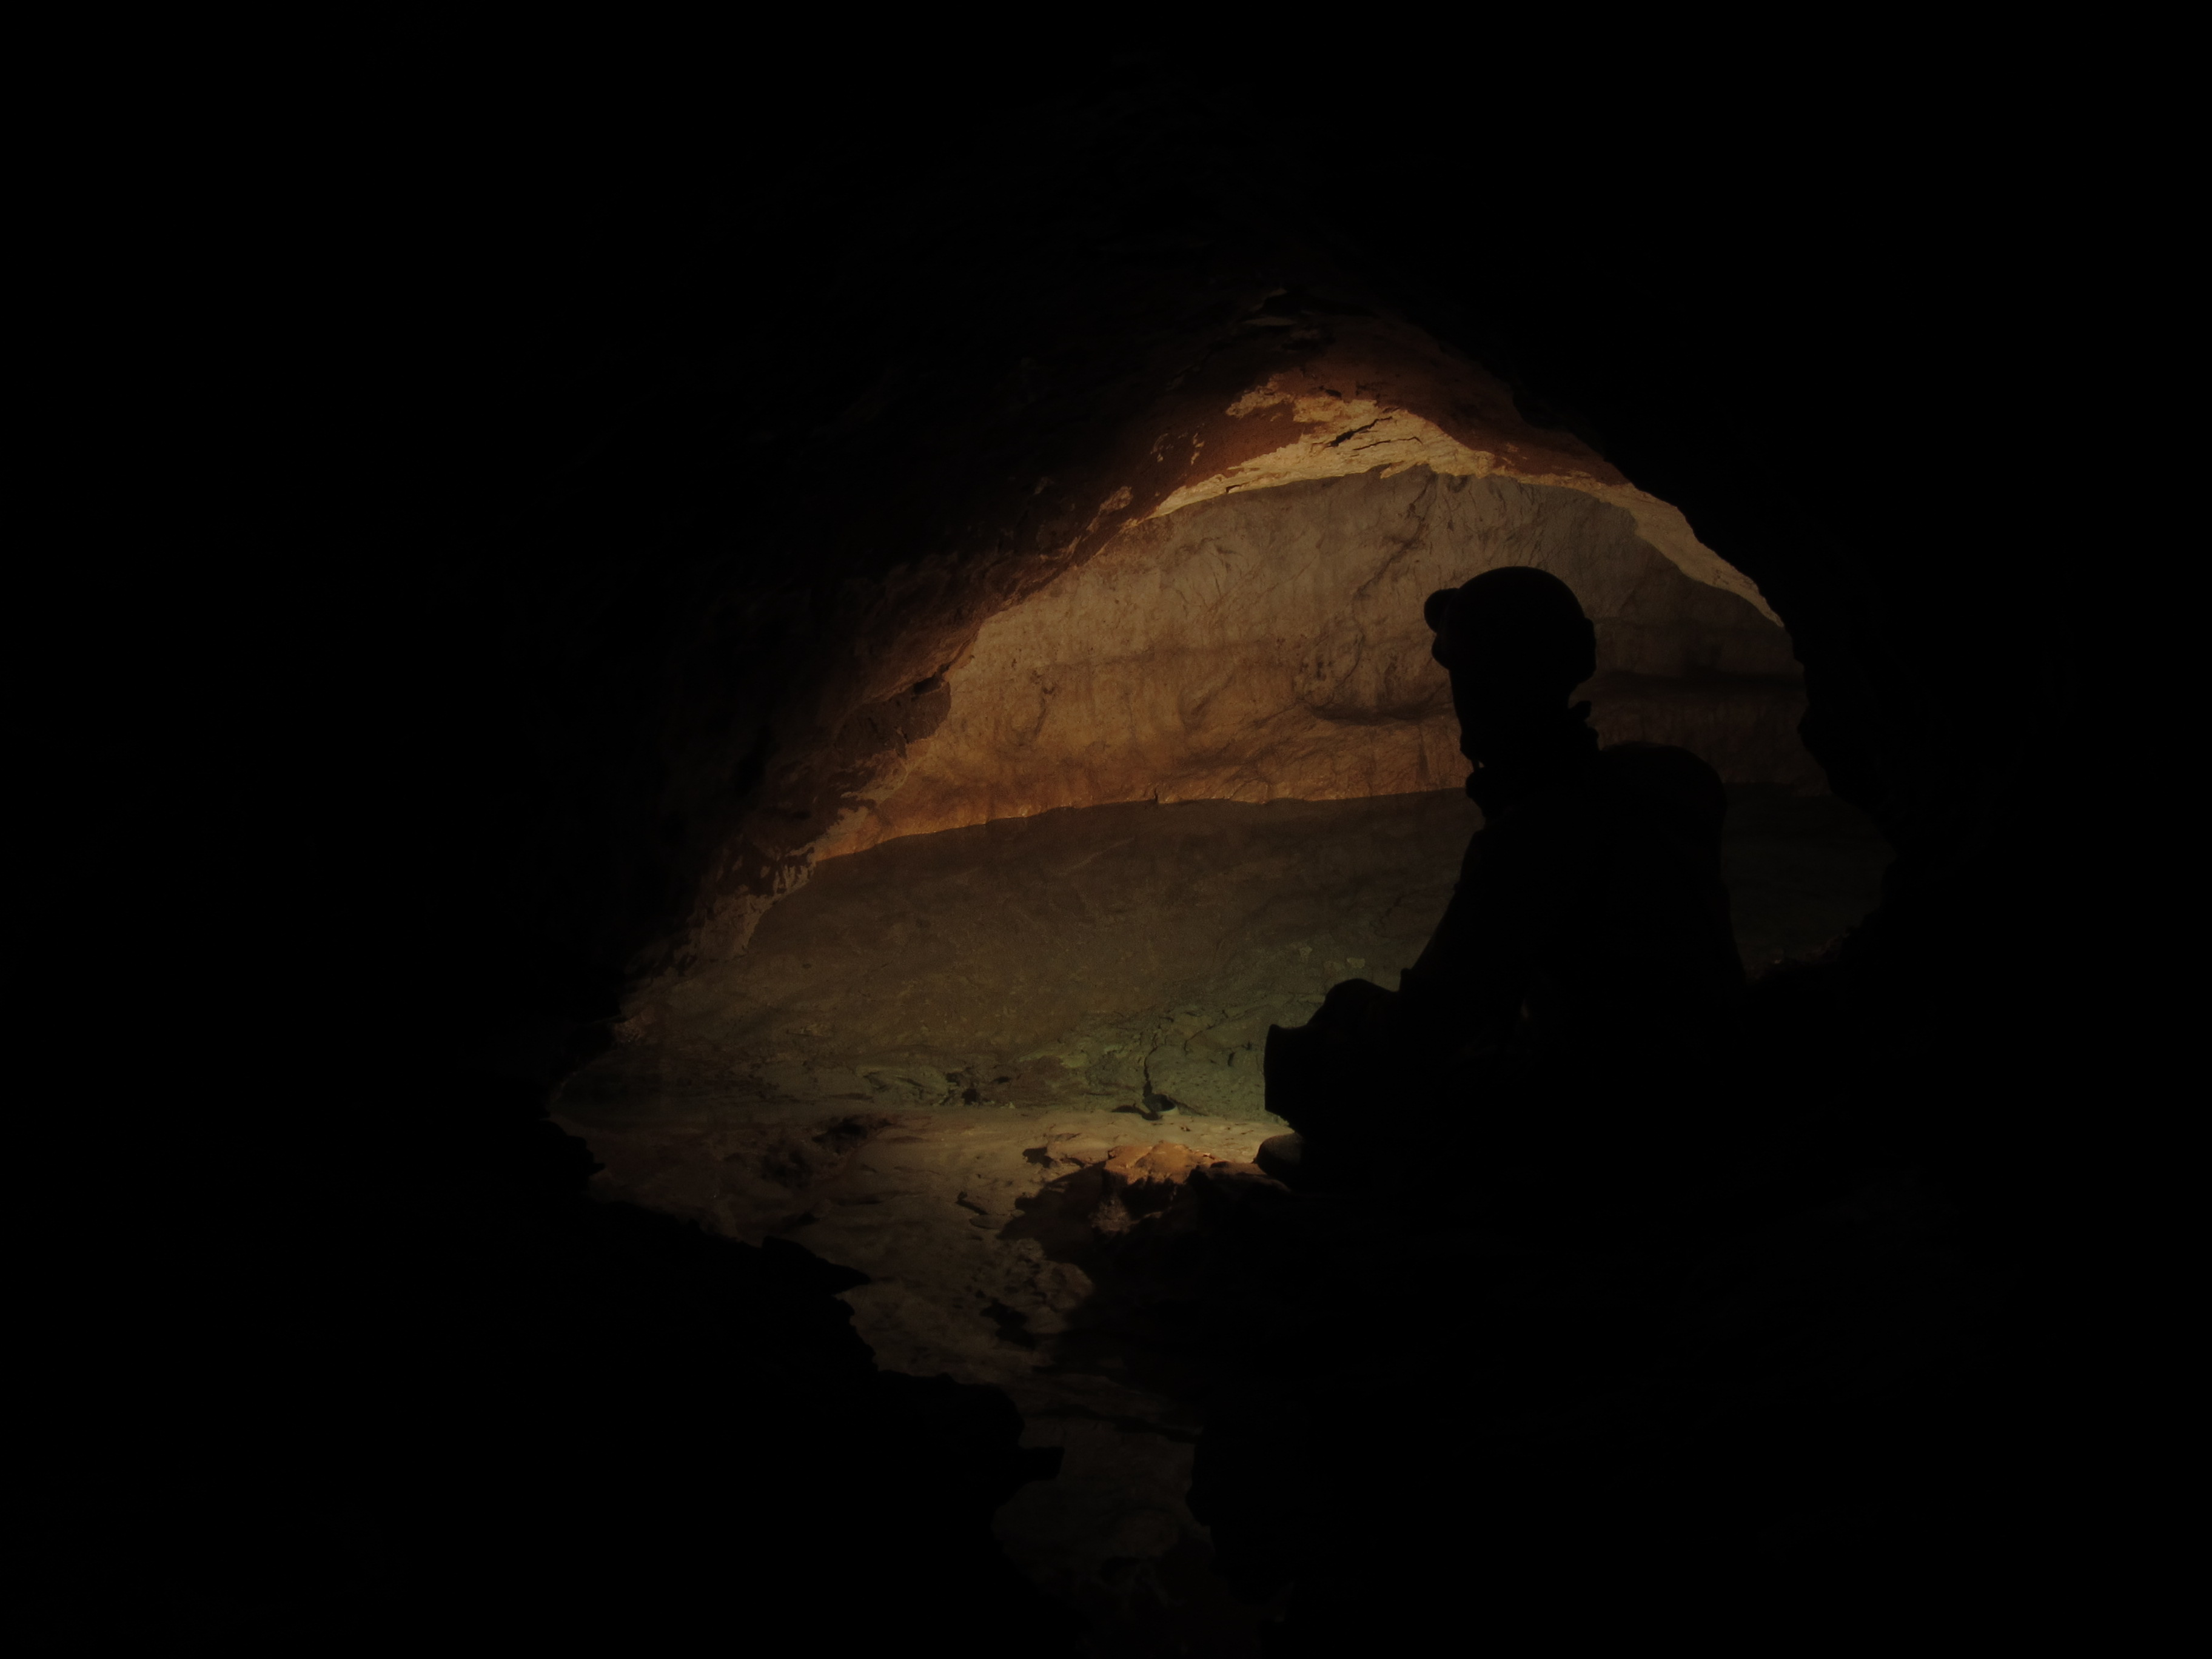
\includegraphics[height=\paperheight]{images/backgrounds/Red_Cow_Sump.jpg}
  					}
	}
\BgThispage
